\documentclass[]{article}

\usepackage{listings}	
\usepackage{float}
\usepackage{graphicx}

\usepackage{titling}
\newcommand{\subtitle}[1]{%
  \posttitle{%
    \par\end{center}
    \begin{center}\large#1\end{center}
    \vskip0.5em}%
}

\begin{document}

\title{Lab 2}
\subtitle{CS M152A}
\author{Aman Agarwal \& Lowell Bander}

\maketitle
%\tableofcontents \newpage


\section{Introduction}

A linear encoding of bits can be interpreted many different ways, for example as unsigned integers, signed integers in 2's complement, and even as floating point values. In this lab we learn how to convert bits in 2's complement to a simple floating point representation.

The input is a 12-bit 2's complement signed integer. The output is an 8-bit floating point value. The 8 bits are split up so that the 1st represents the sign, the next 3, the exponenent, and the last 4, the significand.

\begin{displaymath}
V = (-1)^S \times F \times 2^E
\end{displaymath}

Because 2's complement signed integers don't necessarily map directly to floating point values, we must map these to their closest floating point value through the process of rounding. By using the simple rounding rule provided, we are able to get the closest floating point value for each integer. Without rounding, we only get accurate results for about half of the inputs (those that would round down).

\section{Design Description}
\section{Simulation Documentation}
\section{Conclusion}

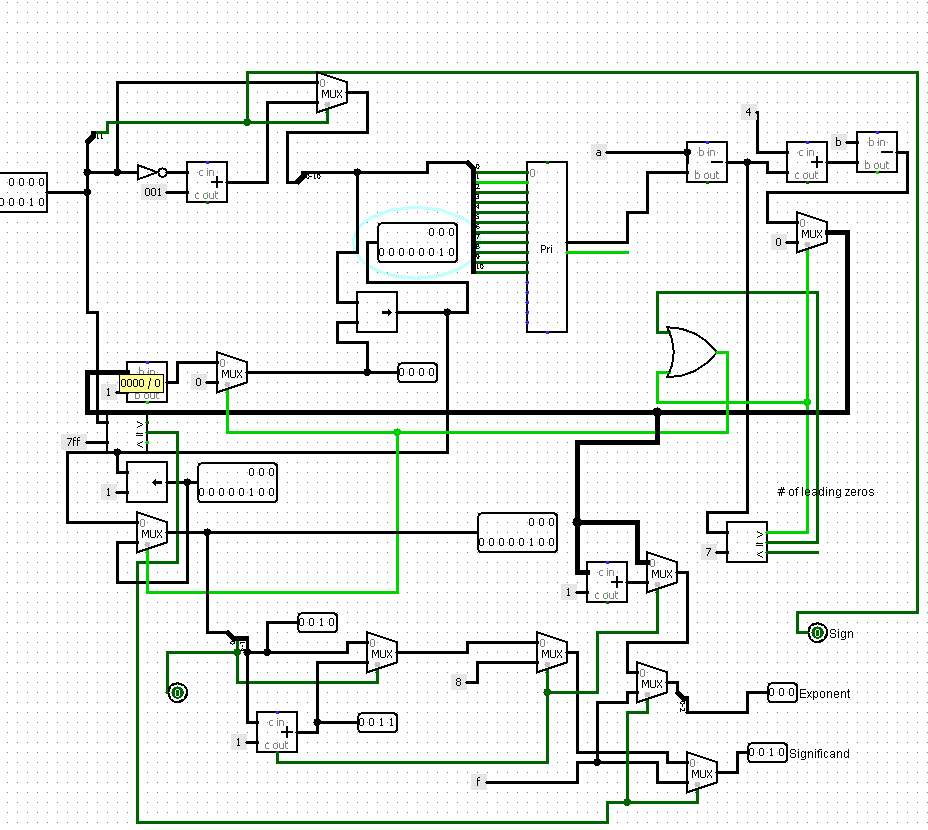
\includegraphics[width=10cm]{logisim.PNG}

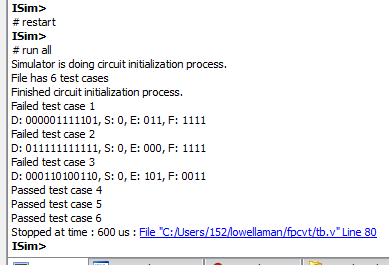
\includegraphics[width=10cm]{output.PNG}

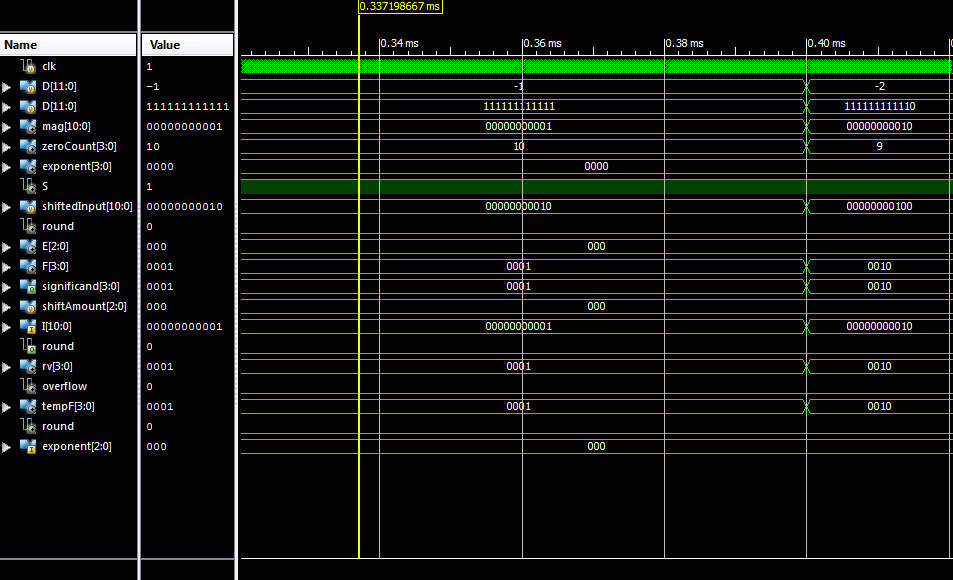
\includegraphics[width=10cm]{waveform.PNG}

\lstinputlisting[language=Verilog, firstline=1, lastline=2]{fpcvt.v}

\lstinputlisting[language=Verilog, firstline=25, lastline=26]{tb.v}


\end{document}

